% Created 2022-07-02 Sat 19:20
% Intended LaTeX compiler: xelatex
\documentclass[11pt,twoside,landscape]{article}
\usepackage{graphicx}
\usepackage{longtable}
\usepackage{wrapfig}
\usepackage{rotating}
\usepackage[normalem]{ulem}
\usepackage{amsmath}
\usepackage{amssymb}
\usepackage{capt-of}
\usepackage{hyperref}
\usepackage{subcaption}
\usepackage[newfloat]{minted}
\usepackage{color}
\usepackage{listings}
\usepackage[top=2cm,bottom=2cm,right=2cm,left=2cm,landscape]{geometry}
\usepackage{multicol}
\usepackage{enumitem}
\usepackage{fancyhdr}
\usepackage{caption}
\usepackage{algorithm}
\usepackage{algpseudocode}
\usepackage{float}
\setlist{noitemsep}
\setlength{\parindent}{0pt}
\setlength{\columnseprule}{0.2pt}
\definecolor{mygreen}{rgb}{0,0.6,0}
\definecolor{mygray}{rgb}{0.5,0.5,0.5}
\definecolor{mymauve}{rgb}{0.58,0,0.82}
\lstset{ backgroundcolor=\color{white}, basicstyle=\footnotesize, breaklines=true, captionpos=b, commentstyle=\color{mygreen}, escapeinside={\%*}{*)},keywordstyle=\color{blue}, stringstyle=\color{mymauve},}
\author{Olivier Lischer}
\date{\today}
\title{ParProg Summary}
\hypersetup{
 pdfauthor={Olivier Lischer},
 pdftitle={ParProg Summary},
 pdfkeywords={},
 pdfsubject={},
 pdfcreator={Emacs 28.1 (Org mode 9.5.4)}, 
 pdflang={English}}
\begin{document}

\pagestyle{fancy}
\fancyhf{}
\fancyhead[R]{ParProg-FS22}
\fancyhead[L]{Exam Summary}
\fancyfoot[CE,CO]{\leftmark}
\fancyfoot[R]{\thepage}
\fancyfoot[L]{Olivier Lischer}

\tableofcontents
\newpage

\begin{multicols}{3}
\section{Multi-Threading Basics}
\label{sec:org938e846}
\subparagraph{async VS. parallel} \
\label{sec:orgc04b3a5}
\emph{Attention}: Asynchron (Concurrent) ist not the same as parallel (see \ref{fig:async-vs-parallel}).
Concurrent means that one core runs multiple threads.
One thread makes progress while the other thread waits for IO.
Parallel means that n cores run n threads at the exactly same time.

{
\begin{center}
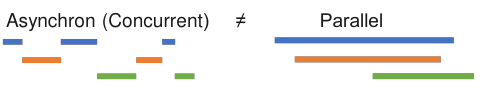
\includegraphics[width=.9\linewidth]{img/async_vs_concurrent.png}
\end{center}
\captionof{figure}{Async vs Parallel}\label{fig:async-vs-parallel}
}

\subparagraph{User-Level Threadings} \
\label{sec:org622226d}
User-Level Threads are implemented in a kind of runtime. 
The runtime itself runs in a process.
Using this approach no real parallelism is possible, only one process).

\subparagraph{Kernel-Level Threading} \
\label{sec:org27c4833}
Today you normally work with Kernel-Level Threads.
The thread mechanism is implemented directly in the kernel.
The programming language only interacts with the kernel API.


{
\begin{center}
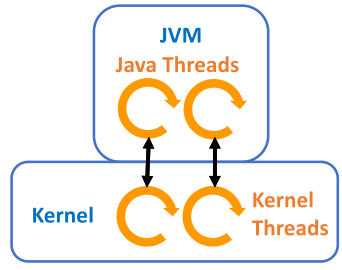
\includegraphics[width=.9\linewidth]{img/kernel_level_threads.png}
\end{center}
\captionof{figure}{Kernel-Level Threads}\label{fig:kernel-level-threads}
}

\subparagraph{Processor Sharing} \
\label{sec:org20cff44}
In modern system you have more threads than processors.
That implies that not every thread can work at any time it wants.
Therefore, the threads must \emph{share} the processor.

\subparagraph{Multi-Tasking} \
\label{sec:org9d795e2}
The processor has two strategies how the processor sharing should work.
\begin{itemize}
\item cooperative
\item preemptive
\end{itemize}

The preemptive is the used model on the processor.
However, the most changes are cooperative because the thread has to wait for other resources (memory, IO, \ldots{}). 

\subparagraph{Cooperative Multi-Tasking} \
\label{sec:orge059019}
In this model the thread works as long as it wants.
If the thread want to wait, it must initiate the process by itself.
A scheduler can not interrupt a running thread!

This model is not very common on modern systems.

\subparagraph{Preemptive Multi-Tasking} \
\label{sec:orge738f93}
The scheduler uses a \emph{Timer Interrupt} to interrupt a running thread.
Each Thread can work for a specific max. interval.
After that interval is over and the thread is not finished, the thread is interrupted and is added to the \emph{Ready-Queue}.

This is the common model which is today used.

\subparagraph{Thread State} \
\label{sec:orge818242}

{
\begin{center}
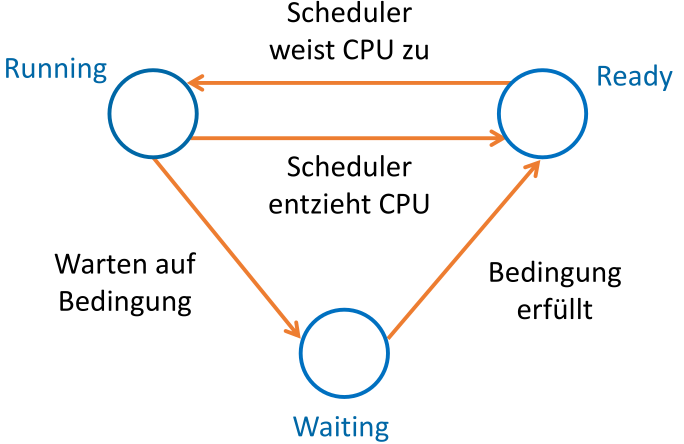
\includegraphics[width=.9\linewidth]{img/thread_states.png}
\end{center}
\captionof{figure}{Thread States}\label{fig:thread-states}
}

\subparagraph{JVM Thread Model} \
\label{sec:org0ec0ca1}
The JVM is a single process system and has many threads (main, daemon threads, \ldots{}).

{
\begin{center}
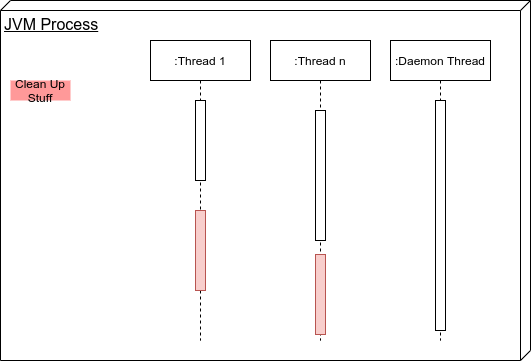
\includegraphics[width=.9\linewidth]{img/jvm_thread_model.drawio.png}
\end{center}
\captionof{figure}{The JVM Thread Model}\label{fig:the-jvm-thread-model}
}

\subparagraph{JVM Termination} \
\label{sec:org1666cda}
The JVM runs as long as at least one non-daemon thread is running.
If the last non-daemon thread is terminated then the JVM is shutdown and all daemon threads are killed uncontrolled.
Therefore, it is not possible to implement something like goodbye message when the thread terminates.

If inside a thread an uncaught exception occurs the other threads are \textbf{not} terminated and keep working.

\subparagraph{InterruptedException Java} \
\label{sec:org3cedd89}
In Java \texttt{join} and \texttt{sleep} can throw (theoretically) a checked \texttt{InterruptedException}.
This exception is never thrown except you call \texttt{myThread.interrupt()}.
Therefore, this exception should only be used if you implement a cooperative canceling.
Otherwise, \texttt{xx.interrupt()} and the exception are indices for a code smell.

\section{Monitor Synchronization}
\label{sec:orgdb29100}
\subparagraph{synchroniyed keyword} \
\label{sec:org53d5174}
In \href{../../../roam/20201116150053-java.org}{Java} every object has a lock called Monitor-Lock.
At the beginning of a \texttt{synchronized} block you acquire the lock as long the lock is free.
If the lock is already acquired then you have to wait.
After the \texttt{synchronized} block the lock is release (in \textbf{every} case)

\lstset{language=java,label= ,caption= ,captionpos=b,numbers=none}
\begin{lstlisting}
public class Test {
    synchronized void do_something() {
	/* do stuff */
    }

    static synchronized void do_other_stuff() { }

}

public class Test2 {
    static void do_other_stuff() {
	synchronized(Test2.class) {}
    }

    void do_something() {
	synchronized(this) {}
    }
}
\end{lstlisting}

\subparagraph{Monitor lock} \
\label{sec:org2ee2ab8}
The monitor is a synchronisation mechanism which use the \emph{Wait \& Signal} mechanism.

\begin{enumerate}
\item Fight for lock
\begin{itemize}
\item winner: enters the monitor (acquire the lock)
\item others: wait for entrance
\end{itemize}
\item Thread in monitor does work
\begin{itemize}
\item if done: leaves monitor and wakes up other threads (\texttt{signal} / \texttt{signalAll()})
\item condition not satisfied: leaves monitor and goes to the right and wake up other threads (Wait on signal)
\end{itemize}
\item Go to 1.
\end{enumerate}


{
\begin{center}
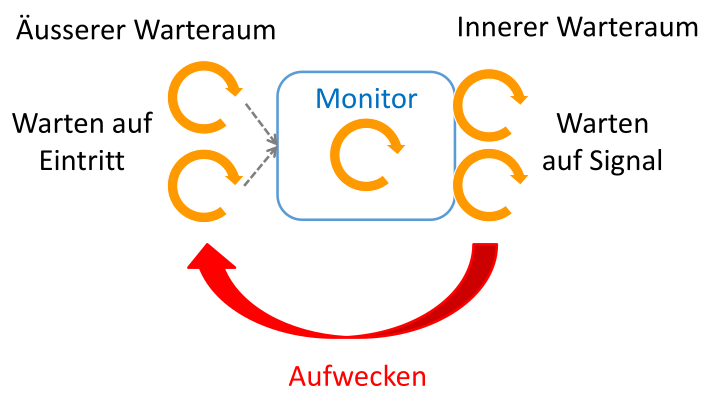
\includegraphics[width=.9\linewidth]{img/monitor.png}
\end{center}
\captionof{figure}{A monitor}\label{fig:monitor}
}

\subparagraph{Wait Function in Loop} \
\label{sec:orgab7b6c3}
The function \texttt{wait()} must be always called inside a loop.
In a simple if condition the following could happen:

\begin{enumerate}
\item thread 1: acquire lock, but condition is not fulfilled -> wait()
\item thread 2: acquire lock, change something, but thread 1 condition not fulfilled
\item thread 1: acquire lock again, make progress even the condition is not fulfilled
\end{enumerate}

\subparagraph{notify vs notifyAll} \
\label{sec:org522f619}
A single notify can only be used when:
\begin{enumerate}
\item every thread has the same condition
\item only one \textbf{single} thread can make progress (One-In/One-Out)
\end{enumerate}

\subparagraph{Thread Wake Up} \
\label{sec:orge76bd2a}
A thread can be woken up by
\begin{enumerate}
\item notifyAll(), notify()
\item InterruptedException
\item Spurious Wake up (falsely wake up POSIX Thread API)
\end{enumerate}

\subparagraph{Implement Monitor Lock} \
\label{sec:org54055da}

\lstset{language=java,label= ,caption= ,captionpos=b,numbers=none}
\begin{lstlisting}
class BankAccount {
    private int balance = 0;

    public synchronized void deposit(int amount) {
	notifyAll();
	balance += amount;
    }

    public synchronized boolean withdraw(int amount) throws InterruptedException {
	int timeout = 0;
	while(amount > balance) {
	    if (timeout >= 3) {
		return false;
	    }
	    wait();
	}

	balance -= amount;
	return true;
    }

    public synchronized int getBalance() {
	return balance;
    }
}

\end{lstlisting}
\section{Specific Synchronization Mechanism}
\label{sec:orge8f475b}
\subparagraph{Semaphore} \
\label{sec:org4cfb27c}
A semaphore is a synchronisation mechanism.
A semaphore is basically a counter which can not count down below 0.

\begin{itemize}
\item \texttt{acquire()}:
\begin{itemize}
\item acquire resource from semaphore
\item wait, as long the counter is <= 0
\item otherwise, decrease counter
\end{itemize}
\item \texttt{release()}:
\begin{itemize}
\item release ressource
\item increment counter
\end{itemize}
\end{itemize}

\subparagraph{Lock and Condition} \
\label{sec:org19c71ef}
In lock \& condition you have a monitor, but instead of one queue you have a queue for each condition.
This has the benefit that not always all threads must be woken up.
Only the threads where the condition may be now fulfilled.

{
\begin{center}
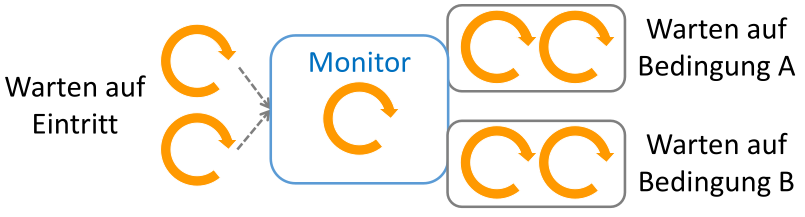
\includegraphics[width=.9\linewidth]{img/lock_and_conditions.png}
\end{center}
\captionof{Lock & Condition}\label{fig:lock-and-conditions}
}

\subparagraph{Lock and Condition Example} \
\label{sec:orgbaffbca}
\lstset{language=java,label= ,caption= ,captionpos=b,numbers=none}
\begin{lstlisting}
import java.util.concurrent.locks.Condition;
import java.util.concurrent.locks.Lock;
import java.util.concurrent.locks.ReentrantLock;

public class WarehouseWithLockCondition {
    private Lock lock;
    private Condition nonEmpty;
    private Condition nonFull;

    public WarehouseWithLockCondition(int capacity, boolean fair) {
	this.capacity = capacity;
	store = 0;
	lock = new ReentrantLock(fair);
	nonEmpty = lock.newCondition();
	nonFull = lock.newCondition();
    }

    @Override
    public void put(int amount) throws InterruptedException {
	lock.lock();
	try {
	    while (store + amount > capacity) {
		nonFull.await();
	    }
	    store += amount;
	    nonEmpty.signalAll();
	} finally {
	    lock.unlock();
	}
    }

    @Override
    public void get(int amount) throws InterruptedException {
	lock.lock();
	try{
	    while (store - amount < 0) { nonEmpty.await(); }
	    store -= amount;
	    nonFull.signalAll();
	}
	finally {
	    lock.unlock();
	}
    }
}
\end{lstlisting}

\subparagraph{Read-Write Locks} \
\label{sec:orgb53f82b}
Mutual exclusion is too strong when only reading happens.
Mutual exclusion is only required when minimal one thread wants to write.

\begin{center}
\begin{tabular}{lll}
Parallel & Read & Write\\
Read & Yes & No\\
Write & No & No\\
\end{tabular}
\end{center}


\lstset{language=java,label= ,caption= ,captionpos=b,numbers=none}
\begin{lstlisting}
var rwLock = new ReentrantReadWriteLock(true);
rwLock.readLock().lock();
// read-only accesses
rwLock.readLock().unlock();
rwLock.writeLock().lock();
// write (and read) accesses
rwLock.writeLock().unlock();
\end{lstlisting}
\subparagraph{Problems With Read-Write Locks} \
\label{sec:orgba914d1}
The benefit of read-write locks is that you not have always mutual exclusion.
But you can use the read lock only then, when \textbf{NO} write access happens on a shared object.
But in common languages like \href{../../../roam/20201116150053-java.org}{Java} it is not possible to encode the read only property into the API.
However, \href{../../../roam/20200904153952-rust.org}{Rust} encodes the mutability of a function directly into the function arguments.
\subparagraph{Count-Down Latch} \
\label{sec:org010809a}
The count down latch is synchronisation mechanism.
It's a counter which counts down to zero.

Using \texttt{await()} you wait until the counter is 0.
Using \texttt{countDown()} you decrement the counter.

\lstset{language=java,label= ,caption= ,captionpos=b,numbers=none}
\begin{lstlisting}
CountDownLatch waitForAll = new CountDownLatch(this.CARS);
protected void waitForAllToBeReady() throws InterruptedException {
    waitForAll.await();
}

@Override
public void readyToStart() {
    waitForAll.countDown();
}
\end{lstlisting}
\subparagraph{Cyclic Barrier} \
\label{sec:org5d56cb0}
A cyclic barrier is a synchronisation mechanism.
The cyclic barrier is a meeting point for a fixed number of threads.
You wait with the function \texttt{await()}.
In contrast to the count down latch a cyclic barrier can be reused.

\lstset{language=java,label= ,caption= ,captionpos=b,numbers=none}
\begin{lstlisting}
var gameRound = new CyclicBarrier(5);

/* 5 different players / threads */
while (true) {
    gameRound.await();
}
\end{lstlisting}


{
\begin{center}
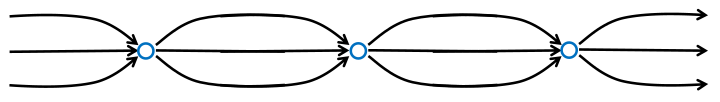
\includegraphics[width=.9\linewidth]{img/cyclic_barrier.png}
\end{center}
\captionof{figure}{Cyclic Barrier}\label{fig:cyclic-barrier}
}
\subparagraph{Rendez-Vous} \
\label{sec:orgdadc91b}
A rendez-vous is a special type of cyclic barrier with only 2 participants.
Often you want to exchange data between those two threads.
For this an \texttt{Exchanger} is used.


\begin{itemize}
\item Without exchange: \texttt{new CyclicBarrier(2);}
\item With exchange: \texttt{Exchanger.exchange(something)};
\end{itemize}


{
\begin{center}
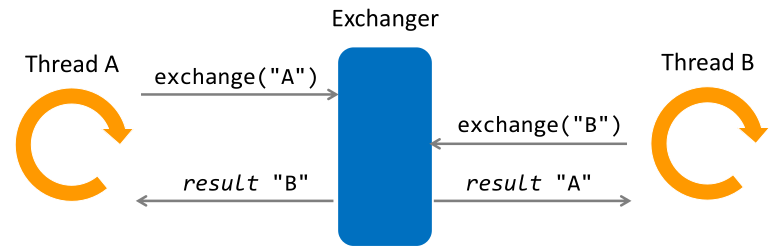
\includegraphics[width=.9\linewidth]{img/exchanger.png}
\end{center}
\captionof{figure}{Exchanger Workflow}\label{fig:exchanger-workflow}
}

\section{Threats of Concurrency}
\label{sec:org5abf9ad}
\subparagraph{Race Conditions} \
\label{sec:orge2e0b20}
A race condition occurs then when multiple threads try to access the same resource without proper synchronization.
This could result in wrong results or wrong behaviour.
Often the reason is a data race.
However, not always.

\subparagraph{Deadlock} \
\label{sec:orga1d707a}
A deadlock is when two or more threads waits on each other.
This happens when thread 1 locks resource \emph{a} and then resource \emph{b} and thread 2 first resource \emph{b} and then resource \emph{a}.

\lstset{language=java,label= ,caption= ,captionpos=b,numbers=none}
\begin{lstlisting}
/* Thread 1 */
synchronized(listA) {
    synchronized(listB) {
	listB.addAll(listA);
    }
}

/* Thread 2 */
synchronized(listB) {
    synchronized(listA) {
	listA.addAll(listB);
    }
}

\end{lstlisting}

{
\begin{center}
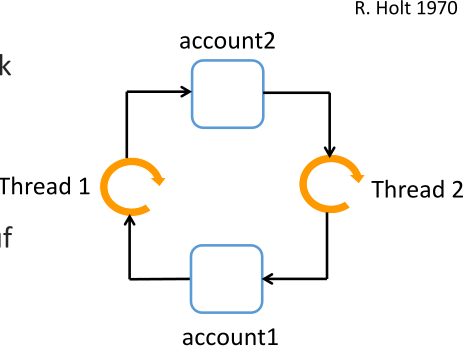
\includegraphics[width=.9\linewidth]{img/deadlock_graph.png}
\end{center}
\captionof{figure}{Deadlock detecion using resource graph}\label{fig:deadlock-detecion-using-resource-graph}
}

\subparagraph{Starvation} \
\label{sec:org5f4a671}
When a thread never can acquire the lock for a resource, even when the lock is release from time to time, we call this \emph{starvation}.
Therefore, it is \textbf{not} a deadlock but a fairness problem.

\subparagraph{Data Race} \
\label{sec:orgcc95304}
When unsynchronized access happens (Race Condition) on the same memory location we call this a data race.
For example, when a thread reads from a variable and another thread writes to the same variable.
A read-read access is \textbf{not} data race (it is also not dangerous).


\lstset{language=java,label= ,caption= ,captionpos=b,numbers=none}
\begin{lstlisting}
/* Thread 1*/
balance += 100;

/* Thread 2*/
balance += 50;
\end{lstlisting}
\subparagraph{Race Condtion withoput data race} \
\label{sec:org651eae2}
In the following code example we see, that no data race is possible.
However, a race condition is still possible.
The read and the subsequent write are not atomic.
The thread can be interrupted between the read and write action.
And the action from another thread gets lost (Lost Update).

\lstset{language=java,label= ,caption= ,captionpos=b,numbers=none}
\begin{lstlisting}
class BankAccount {
    int balance = 0;
    synchronized int getBalance() { return balance; }
    synchronized void setBalance(int x) { balance = x; }
}

/* On multiple threads */
account.setBalance(account.getBalance() + 100);
\end{lstlisting}
\subparagraph{No synchronization needed} \
\label{sec:org18bbf7e}
Synchronization is not required when:
\begin{itemize}
\item the object is immutable (read only access)
\item with confinement
\end{itemize}

\subparagraph{Confinement} \
\label{sec:org01540b4}
Under confinement, we understand a structure that guaranties that only one thread can access an object at time.
\begin{itemize}
\item \emph{Thread Confinement}: an object belongs to a single thread and is used only be this thread
\item \emph{Object Confinement}: an object is encapsulated in an already synchronized object
\end{itemize}


\lstset{language=java,label= ,caption= ,captionpos=b,numbers=none}
\begin{lstlisting}
class ProductDatabase {
    private HashMap<String, Product> productMap = new HashMap<>();

    public synchronized void addProduct(String name, String details) {
	productMap.put(name, new Product(details));
    }

    public synchronized getProductDetails(String name) {
	return productmap.get(name).getDetails(); // save, because String is immutable
    }

    public synchronized void notifySale(String name) {
	productMap.get(name).increaseSales();
    }
}
\end{lstlisting}


{
\begin{center}
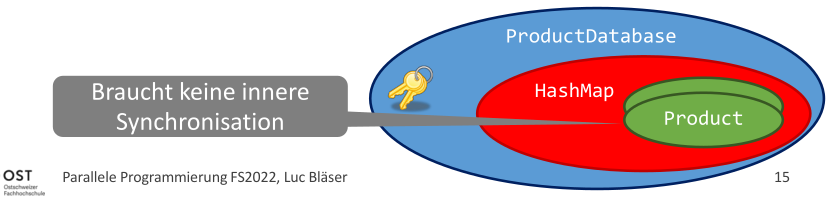
\includegraphics[width=.9\linewidth]{img/object_confinement.png}
\end{center}
\captionof{figure}{Example of object confinement}\label{fig:example-of-object-confinement}
}

\subparagraph{Livelock} \
\label{sec:orgd02ca76}
A live lock is a special case of a deadlock.
While in a deadlock all relevant threads are sleeping in a live lock the threads are doing some waiting instruction.
During these waiting instructions the CPU is working (busy wait).
\subparagraph{Avoiding deadlocks} \
\label{sec:orgd0f23ae}
To avoid deadlocks you have two possibilities:
\begin{itemize}
\item with a linear lock order
\item coarse-grained locking (when linear lock order is not possible)
\end{itemize}


{
\begin{center}
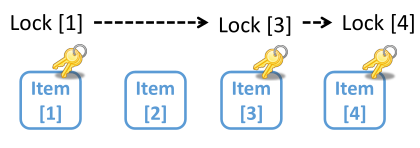
\includegraphics[width=.9\linewidth]{img/linear_lock_order.png}
\end{center}
\captionof{figure}{Linear Lock Order}\label{fig:linear-lock-order}
}

{
\begin{center}
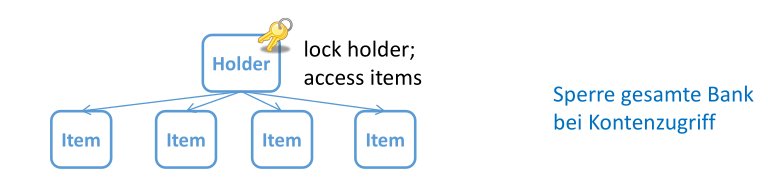
\includegraphics[width=.9\linewidth]{img/coarse_grained_locking.png}
\end{center}
\captionof{figure}{Coarse Grained Lock}\label{fig:coarse-grained-lock}
}
\section{Thread Pools}
\label{sec:org0c61bd9}
\subparagraph{Thead Pool} \
\label{sec:org6832954}
A thread pool consists of a task queue and n worker threads.
A new task is inserted in the queue.
The new free thread from the thread pool takes the first task from the queue and process it.

{
\begin{center}
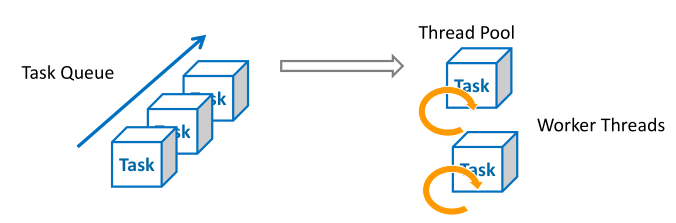
\includegraphics[width=.9\linewidth]{img/thread_pool.png}
\end{center}
\captionof{Thread Pool}\label{fig:thread-pool}
}

\subparagraph{Number of Threads in Thread Pool} \
\label{sec:org7320a67}
A thread pool has as much threads as processors (cores) and little bit more.
A little bit more than the number of processors is ideally because when one thread has to wait for I/O another thread can use the processor:

\begin{equation}
  \begin{align}
    & \text{\#Worker Threads} = \\
    & \text{\#Prozessoren} + \text{\#Pendente I/O-Aufrufe}
  \end{align}
\end{equation}

\subparagraph{Thread Pool Java} \
\label{sec:org910a80d}
Today in modern Java you should only use the \texttt{ForkJoinPool}.
If an exception occures then the exception is returnted to the caller of \texttt{get()}.

\lstset{language=java,label= ,caption= ,captionpos=b,numbers=none}
\begin{lstlisting}
var threadPool = new ForkJoinPool();
// submit is non-blocking
Future<Integer> future = threadPool.submit(() -> {
	int value = 1;
	// long calculation
	return value;
    });

// get blocks / same as await in Rust
Integer i = future.get();
\end{lstlisting}
\subparagraph{Task Parallelism .NET} \
\label{sec:org72142ba}
In \href{../../../roam/20211003114703-net.org}{.NET} you have one thread pool for:
\begin{itemize}
\item task parallelization
\item data parallelization
\item async programming
\end{itemize}

\lstset{language=csharp,label= ,caption= ,captionpos=b,numbers=none}
\begin{lstlisting}
Task task1 = Task.Run(() => { /* Do some stuff */ });
task1.Wait(); // blocking

// Task with return value
Task task2 = Task.Run(() => { return 3;});
Console.Write(task.Result); // blocking

// Task with Sub Tasks
Task.Run(() => {
    var left = Task.Run(() => Count(leftPart));
    var right = Task.Run(() => Count(rightPart));
    int result = left.Result + right.Result;
    return result;
});

// Parallele Statements
Parallel.Invoke(
    () => MergeSort(l, m),
    () => MergeSort(m, r)
);

// Parallel Loop
Parallel.ForEach(list, file => Convert(file));

// Parallel For - only if iterations are indepentend
Parallel.For(0, array.Length, i => DoComputation(array[i]));

// PLINQ
from book in bookCollection.AsParallel()
    where book.Title.Contains("Concurrency")
    select book.ISBN;

from number in inputList.AsParallel().AsOrdered()
    select IsPrime(number);
\end{lstlisting}
\subparagraph{Parallel Loop .NET} \
\label{sec:orgf6132e3}
Often a loop has just a very short body.
It is inefficient to execute every iteration in its own task.
Therefore, the TPL groups automatically multiple bodies to a single task.

{
\begin{center}
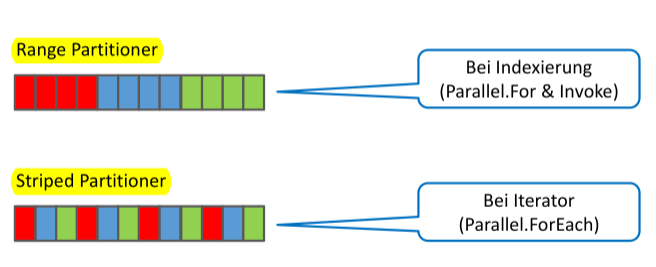
\includegraphics[width=.9\linewidth]{img/partitioning_in_loop_tpl.png}
\end{center}
\captionof{figure}{Partitioning in Parallel Loops}\label{fig:partitioning-in-parallel-loops}
{
\subparagraph{Work Stealing Pool} \
\label{sec:org43adacd}
Each Worker Thread has also its own task queue.
A worker thread takes some task from the global queue and move it to the local queue.
If the another worker thread wants to work but the global queue is empty, it steals it from other worker threads.


{
\begin{center}
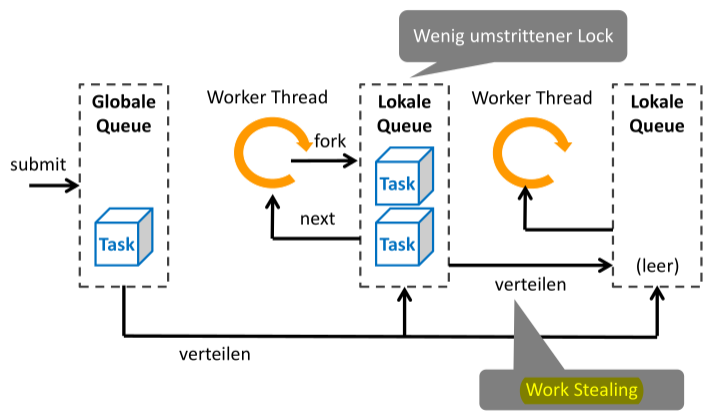
\includegraphics[width=.9\linewidth]{img/work_stealing_thread_pool.png}
\end{center}
\captionof{figure}{Work Stealing Thread Pool}\label{fig:work-stealing-thread-pool}
}
\subparagraph{Thread Injection} \
\label{sec:orgbe6b18d}
When I injection new Threads in the thread pool during runtime is called \emph{Thread Injection}.
This can mitigate possible deadlocks when two task are not indepentend (only if not max threads is set).

\subparagraph{{\bfseries\sffamily TODO} Some Stuff} \
\label{sec:orgc22087a}
\section{Async Programming}
\label{sec:orgf32871e}
\subparagraph{Types of asynchrony} \
\label{sec:orgac3006c}
You differ between two types of asynchrony:
\begin{itemize}
\item caller centric (pull)
\begin{itemize}
\item The caller waits for task end and pulls the result
\end{itemize}
\item callee centric (push)
\begin{itemize}
\item task forwards the result to the successor task
\end{itemize}
\end{itemize}

\subparagraph{Continuation in C\#} \
\label{sec:org417d051}

\lstset{language=csharp,label= ,caption= ,captionpos=b,numbers=none}
\begin{lstlisting}
Task.Run(task1).
    ContinueWith(task2).
    COntinueWith(task3);
\end{lstlisting}

{
\begin{center}
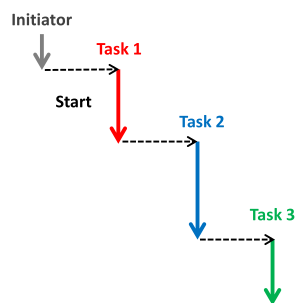
\includegraphics[width=.9\linewidth]{img/task_continuations.png}
\end{center}
\captionof{figure}{Task Continuations}\label{fig:task-continuations}
}


\lstset{language=csharp,label= ,caption= ,captionpos=b,numbers=none}
\begin{lstlisting}
Task.WhenAll(task1, task2).
    ContinueWith(continuation);

Task.WhenAny(task1, task2).
    ContinueWith(continuation);
\end{lstlisting}

{
\begin{center}
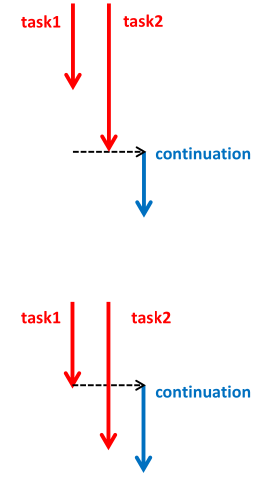
\includegraphics[width=.9\linewidth]{img/task_multi_continuation.png}
\end{center}
\captionof{figure}{Multi Continuation}\label{fig:multi-continuation}
}

\subparagraph{Exception Handling Continuation} \
\label{sec:orgb53291a}
Exception in a Fire \& Forget Tasks are ignored.

\lstset{language=csharp,label= ,caption= ,captionpos=b,numbers=none}
\begin{lstlisting}
Task.Run(() => {
    throw new Exception("Some text"); // This exception is ignored by the system
});
\end{lstlisting}

To handle exceptions you could wait synchrony for finishing the task continuations (listening \ref{lst:synchron-wait-for-finishing-task-continuation}).
Another option would be to subscribe for the \texttt{UnobservedTaskException}.
However, this event is only triggered when the task is clean upped by the \href{../../../roam/20211008083744-garbage_collection.org}{Garbage Collection}.
This can be at every point in time or even never (not deterministic).

\lstset{language=csharp,label=lst:synchron-wait-for-finishing-task-continuation,caption={Synchron Wait for finishing task continuation},captionpos=b,numbers=none}
\begin{lstlisting}
task1.
    ContinueWith(task2).
    ContinueWith(task3).
    Wait();
\end{lstlisting}
\subparagraph{CompletableFuture Java} \
\label{sec:org084bca7}
\texttt{CompletableFuture} is how you write async programs in modern \href{../../../roam/20201116150053-java.org}{Java} and is the Java part of \texttt{Task} from C\#.

The \texttt{CopletableFuture} has the methods listed in \ref{tbl:methods-for-async-programming}. 

\begin{table}[htbp]
\caption{\label{tbl:methods-for-async-programming}Methods for async programming}
\centering
\begin{tabular}{lll}
 & void operation & with return value\\
\hline
Async Call & \texttt{runAsync} & \texttt{supplyAsync}\\
Continuation & \texttt{thenAccept} & \texttt{thenApply}\\
\end{tabular}
\end{table}

For Multi Continuation you have the following methods:
\begin{itemize}
\item \texttt{CompletableFuture.allOf(future1, future2)}
\item \texttt{CompletableFuture.any(future1, future2)}
\end{itemize}


Other than .NET you can perform proper exception handling in continuations with \texttt{exceptionally()}.

\subparagraph{Update UI .NET} \
\label{sec:org2b95101}
In \href{../../../roam/20211123162923-wpf.org}{WPF} only the UI Thread is allowed to update the UI.
Using a Dispatcher you can run an operation on the UI Thread from the background.
In a WPF Project you can access the dispatcher:
\begin{itemize}
\item Code Behind: \texttt{this.Dispatcher}
\item Other classes: \texttt{Application.Current.Dispather}
\end{itemize}
\subparagraph{Aysnc in .NET} \
\label{sec:orgee58770}
A async function in \href{../../../roam/20211003114703-net.org}{.NET} can only have the following return types:
\begin{itemize}
\item \texttt{Task}
\item \texttt{Task<T>}
\item \texttt{void} (fire and forget, should only be used in exceptional cases)
\end{itemize}


{
\begin{center}
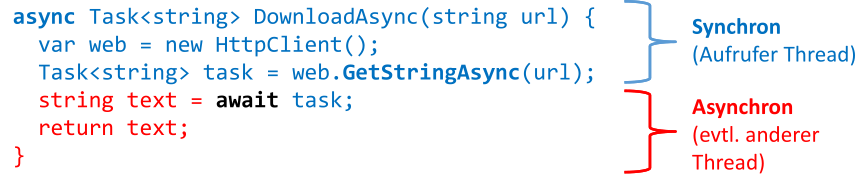
\includegraphics[width=.9\linewidth]{img/async_await_execution_modell.png}
\end{center}
\captionof{figure}{Async / Await Execution Modell}\label{fig:async-await-execution-modell}
}

\subparagraph{async / await execution model .NET} \
\label{sec:org1fb843d}
The compiler splits the async function in multiple parts:
\begin{enumerate}
\item section before await: this section is executed synchrony
\item section after await: This is executed \textbf{after} the task is finished as a continuation.
\end{enumerate}


{
\begin{center}
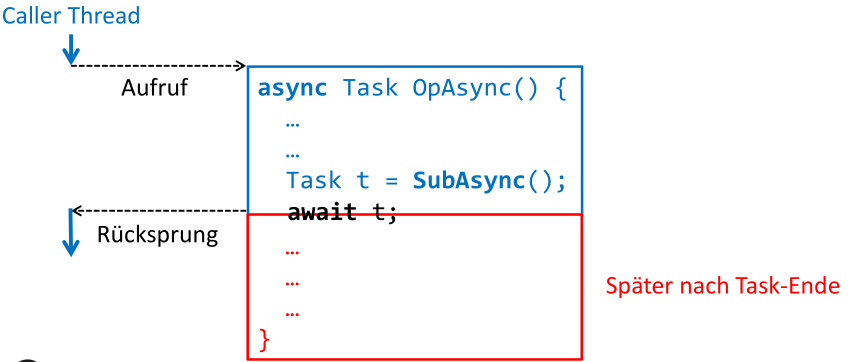
\includegraphics[width=.9\linewidth]{img/async_method_call.png}
\end{center}
\captionof{figure}{Async Method Call}\label{fig:async-method-call}
}

\begin{figure}[H]
  \centering
  \begin{subfigure}{0.4\textwidth}
    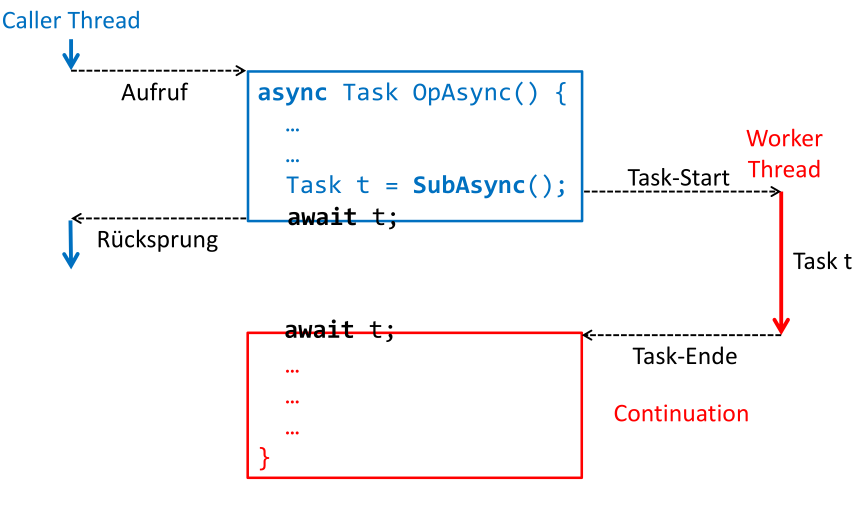
\includegraphics[width=3in]{img/non_ui_thread.png}
    \caption{Non-UI Thread Execution \label{fig:non-ui-thread-execution}}
  \end{subfigure}
  \hfill
  \begin{subfigure}{0.4\textwidth}
    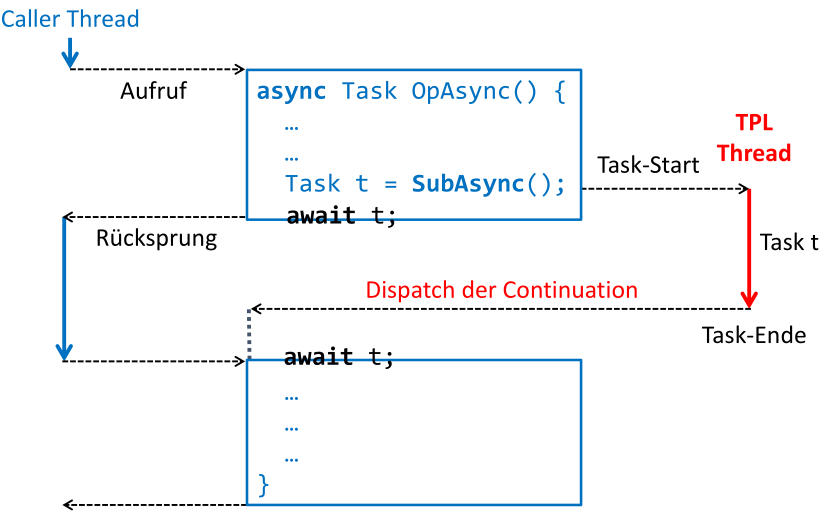
\includegraphics[width=3in]{img/ui_thread.png} 
    \caption{UI Thread Execution \label{fig:ui-thread-execution}}
  \end{subfigure}
  \caption{
    \label{fig:thread-execution}
    Thread Execution
  }
\end{figure}

\section{Memory Model}
\label{sec:org97ff05a}
\subparagraph{Lock Free Programming} \
\label{sec:orga6f74ca}
Lock Free Programming is a type of programming where you write concurrent programs without any lock mechanism.
In lock free programming you use the guaranties of the memory model.
The goal of lock free programming is to create efficient synchronization.

\subparagraph{Weak Consistency} \
\label{sec:orgbb39073}
The memory access to the same memory address is seen differently by different threads.
The possible output for j and i in \ref{fig:example-for-weak-consitency-example} are:
\begin{itemize}
\item i = 0, j = 0
\item i = 1, j = 1
\item i = 0, j = 1
\item i = 1, j = 0
\end{itemize}


{
\begin{center}
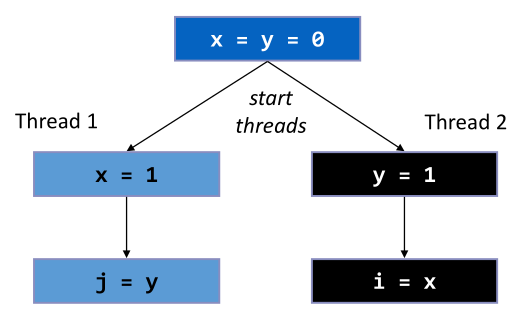
\includegraphics[width=.9\linewidth]{img/weak_consistency_example.png}
\end{center}
\captionof{figure}{Example for Weak Consitency Example}\label{fig:example-for-weak-consitency-example}
}

The reason for this is that the compiler, runtime systems, CPUs, etc. can reorder instructions for optimization purpose.
\textbf{Expect}, you use synchronization or memory barriers.
This is called \textbf{weak consistency}.

\subparagraph{Atomicity Guaranty Java} \
\label{sec:orga440ac5}
Single reads / writes are atomic for:
\begin{itemize}
\item primitive data types until 32 bits
\item object references
\item long and double only with the \texttt{volatile} keyword
\end{itemize}

\subparagraph{Visibility Guaranty Java} \
\label{sec:org095ef93}

Java guaranties the following visibility:
\begin{itemize}
\item changes before release are visible at acquire (\ref{fig:visibility-lock-unlock})
\item changes until write are visible at read (\ref{fig:visibility-volatile-write-read})
\item the thread sees the correct start values and Join the output of the thread
\item initialization of final variables (only relevant if you get the object from a data race!)
\end{itemize}


{
\begin{center}
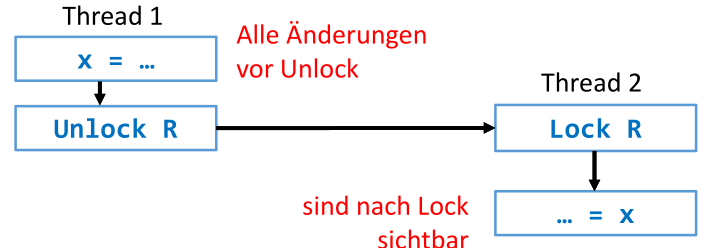
\includegraphics[width=.9\linewidth]{img/visibility_lock_unlock.png}
\end{center}
\captionof{figure}{Visibility Lock / Unlock}\label{fig:visibility-lock-unlock}
}

{
\begin{center}
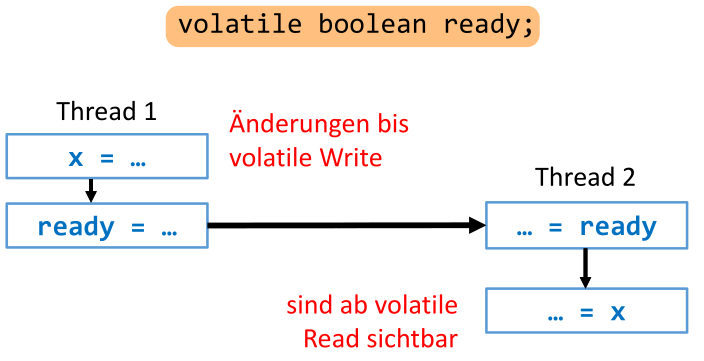
\includegraphics[width=.9\linewidth]{img/visibility_volatile_write_read.png}
\end{center}
\captionof{figure}{Visibility Volatile Write / Read}\label{fig:visibility-volatile-write-read}
}


{
\begin{center}
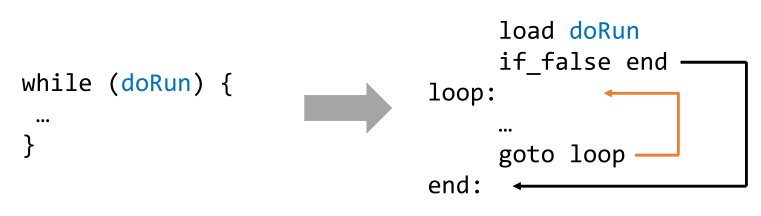
\includegraphics[width=.9\linewidth]{img/visibility_problems.png}
\end{center}
\captionof{figure}{Visibility Problems}\label{fig:visibility-problems}
}
\subparagraph{Ordering Guaranty Java} \
\label{sec:orgf464275}
The order of the visibility is the same as in visibility.
Additional:
\begin{itemize}
\item synchronization instructions are never reordered to each other
\item Lock/Unlock, volatile, thread start / join are never reordered
\item if everything is a synchronization mechanism than we talk about total order
\end{itemize}


{
\begin{center}
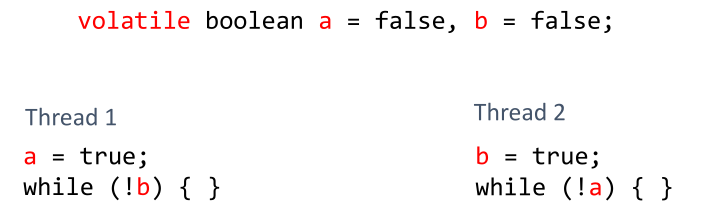
\includegraphics[width=.9\linewidth]{img/total_order.png}
\end{center}
\captionof{figure}{Total Order Rendez-Vous}\label{fig:total-order-rendez-vous}
}
\subparagraph{Atomic Actions Java} \
\label{sec:org9c7d558}
Java has for each type an Atomic class.
This class provides many functions which are atomic.
\begin{itemize}
\item \texttt{getAndSet()}
\item \texttt{compareAndSet()}
\item \texttt{set()}
\item \ldots{}
\end{itemize}

\subparagraph{Optimistic Synchronization Java} \
\label{sec:orge5c3046}
In optimistic synchronization you perform the operation on a snapshot.
If the snapshot is still the same value after the (long) operation you can update it.
Otherwise, you have to do the same steps again until the fetch value is equal.

\lstset{language=java,label= ,caption= ,captionpos=b,numbers=none}
\begin{lstlisting}
do {
    oldValue = var.get();
    newValue = caculateChanges(oldValue);
} while(!var.compareAndSet(oldValue, newValue));


// possible implementation for updateAndGet on the AtomicXXX
void updateAndGet(lambda calculateChanges) {
    do {
	oldValue = this.get();
	newValue = calculateChanges(oldValue);
    } while (!var.compareAndSet(oldValue, newValue));
}
\end{lstlisting}

\subparagraph{.NET Memory Model} \
\label{sec:org713f9c0}
In general the .NET Memory Model is the same as in Java with a few exepctions:
\begin{itemize}
\item atomicity: long / double are not atomic, event with volatile
\item visibility: not defined, implicit defined by ordering
\item ordering: only half and full fences
\end{itemize}


The .NET version of the Atomic classes in \href{../../../roam/20201116150053-java.org}{Java} is the \texttt{Interlocked} class.


\lstset{language=csharp,label=fig:net-full-fence,caption={.NET Full Fence},captionpos=b,numbers=none}
\begin{lstlisting}
Thread.MemoryBarrier();
\end{lstlisting}


{
\begin{center}
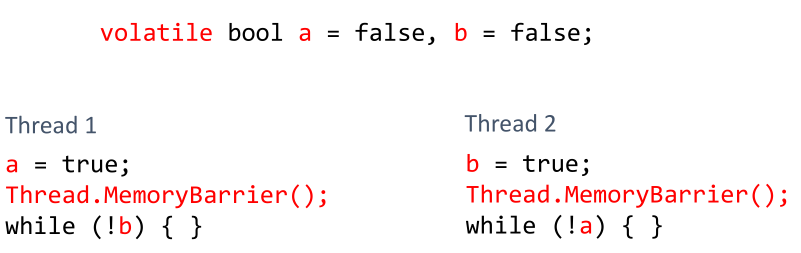
\includegraphics[width=.9\linewidth]{img/rendez_vous_in_net.png}
\end{center}
\captionof{figure}{Rendez-Vous in .NET}\label{fig:rendez-vous-in-net}
}
\subparagraph{Volatile Half Fences .NET} \
\label{sec:org5e82248}
The \texttt{volatile} keyword in .NET is only a Half Fence.
That means
\begin{itemize}
\item volatile writes: previous access stay before
\item volatile reads: following access remain after
\end{itemize}

{
\begin{center}
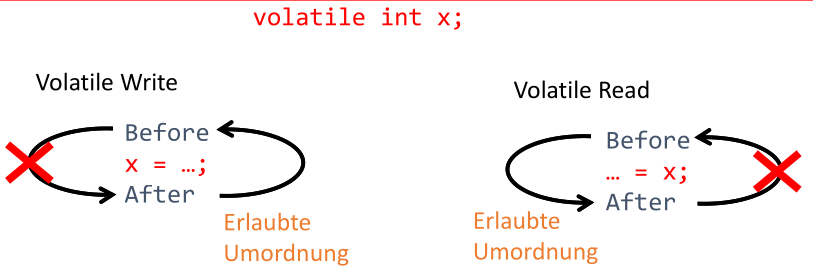
\includegraphics[width=.9\linewidth]{img/net_volatile_half_fences.png}
\end{center}
\captionof{figure}{.NET Volatile Half Fences}\label{fig:net-volatile-half-fences}
}
\section{GPU Parallelization:}
\label{sec:org5a35fbe}
\subparagraph{Lacency vs throughput} \
\label{sec:orgc767db5}
\begin{description}
\item[{latency}] how long does it take to execute a single instruction / operation
\item[{throughput}] number of instructions / operations completed per second
\end{description}

High throughput: lots of pizzas per hour
\subparagraph{compute \& memory bound} \
\label{sec:org2db0e37}
The performance of a function is defined by memory bandwidth, compute bandwidth and latency.
Total time for a function is \texttt{memory access + compute time}.
If the compute time takes longer we say the function is \emph{compute bound}.
If the memory time takes longer we say the function is \emph{memory bound}.

\subparagraph{When to use the GPU} \
\label{sec:orgd15cc58}
The GPU is good if you can run the same instruction on multiple data at the same time.
Therefore, GPU parallelism is only then a good idea when the function / code is compute bound.
If the problems is the memory access then it is not a good idea to use the GPU.

\subparagraph{Arithmetic Intensity} \
\label{sec:org5d55a74}
The arithmetic intensity describes the ration between computing and memory access.
The higher, the better: efficient utilization of modern parallel processors.

\begin{equation}
  \begin{align}
    &t_c > t_m \\
    &\frac{ops}{BW_c} > \frac{bytes}{BW_m} \\
    &\frac{ops}{bytes} > \frac{BW_C}{BW_m} \\
    &\text{Arithmetic intensity} = \frac{BW_c}{BW_m}
  \end{align}
\end{equation}

If your arithmetic intensity is low, then you may not want to use the GPU.
Instead, you want to optimize the memory access.

\subparagraph{Roof line model} \
\label{sec:orgec0b1ba}

The roof line model describes visually where your applications has performance issues.

In point O\textsubscript{1} we can not fully use the GPU because the memory is too slow.
However, in O\textsubscript{2} the CPU is can not calculate faster and in this point it is a good idea to use \href{../../../roam/20220518173241-gpu.org}{GPU}. 


{
\begin{center}
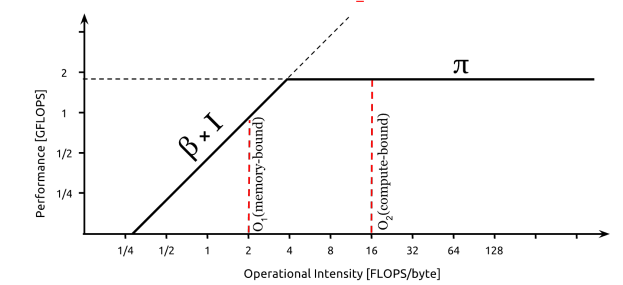
\includegraphics[width=.9\linewidth]{img/roof_line_model.png}
\end{center}
\captionof{figure}{Roof line model}\label{fig:roof-line-model}
}

\subparagraph{GPU Structure} \
\label{sec:orgca5bead}
The big difference between the CPU and the \href{../../../roam/20220518173241-gpu.org}{GPU} are the numbers of transistors for computing.
The GPU has a lot more, but they are that good as the CPU ones.

A GPU consists of many \textbf{Streaming Multiprocessors (SM)}.
And each SM consist of many \textbf{Streaming Processors (SP)} (Cores).


{
\begin{center}
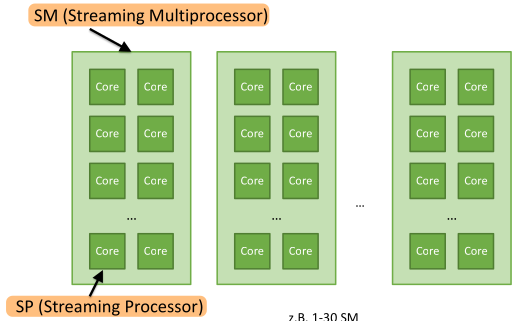
\includegraphics[width=.9\linewidth]{img/gpu_structure.png}
\end{center}
\captionof{GPU structure}\label{fig:gpu-structure}
}

\subparagraph{SIMD} \
\label{sec:org71a206f}
Single Instruction Multiple Data (SIMD) is performed on a Streaming Multiprocessor.
Each core performs the exact same instructions but with different data.

{
\begin{center}
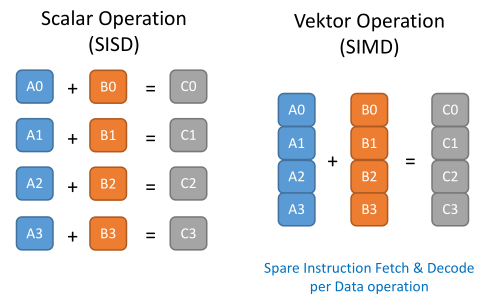
\includegraphics[width=.9\linewidth]{img/simd_vector_parallelism.png}
\end{center}
\captionof{figure}{SIMD Vector parallelism}\label{fig:simd-vector-parallelism}
}

\subparagraph{NUMA} \
\label{sec:org01b8554}
The NUMA model (Non-Uniform Memory Access) describes a model where two processors (CPU or GPU) do \textbf{NOT} share the memory.
Therefore, one processor has to copy the data into other memory and back from there.
The access time to the local memory (on-device) is much faster than the access to the remote one.

{
\begin{center}
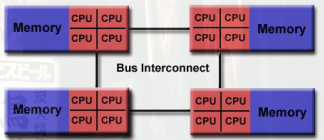
\includegraphics[width=.9\linewidth]{img/numa_model_cpu.png}
\end{center}
\captionof{figure}{The NUMA model}\label{fig:the-numa-model}
}

\subparagraph{Thermilogy} \
\label{sec:org2f3be05}

\begin{center}
\begin{tabular}{lll}
CUDA & OpenCL & Desc\\
\hline
Kernel & Kernel & Function to run on GPU\\
Host Program & Host Program & Application which calls the kernel on the GPU\\
Thread & Work Item & A single thread which runs on the GPU\\
Block & Work Group & A collection of threads running simultaneously (SM)\\
Grid & NDRange & A collection of blocks\\
\end{tabular}
\end{center}


{
\begin{center}
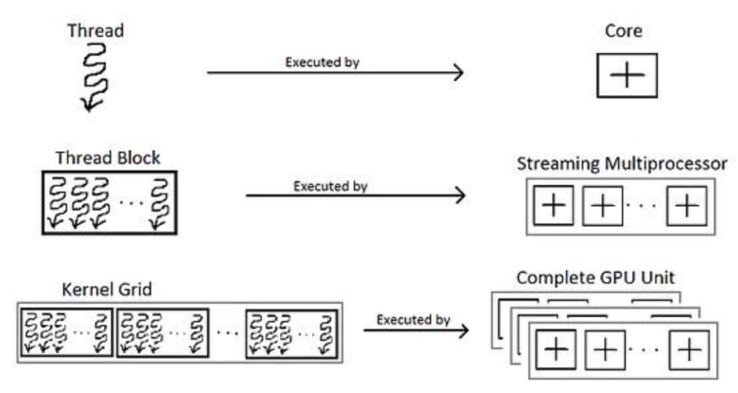
\includegraphics[width=.9\linewidth]{img/cuda_to_gpu_analogy.png}
\end{center}
\captionof{figure}{CUDA concepts on the GPU}\label{fig:cuda-concepts-on-the-gpu}
}

\subparagraph{Thread Hierarchy} \
\label{sec:org5a812a5}
A Kernel is executed in a single thread.
The single thread is executed simultaneously to other threads in a block.
Many blocks are executed at the same time on a grid.

Internally, the threads are grouped into warps.
Theses, are executed in a block.

Important: Each block can only execute a specific number of threads.
And a grid can only execute a specific number of blocks.


{
\begin{center}
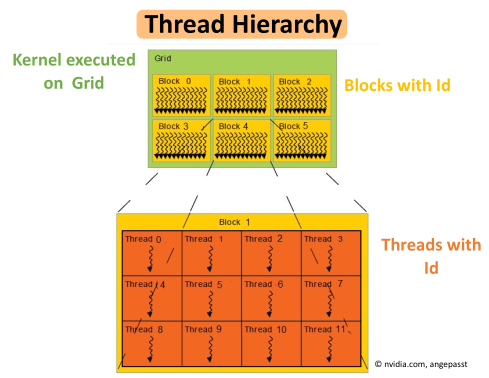
\includegraphics[width=.9\linewidth]{img/thread_hierarchy.png}
\end{center}
\captionof{figure}{Thread Hierarchy on GPU}\label{fig:thread-hierarchy-on-gpu}
}

\section{Performance Optimizations}
\label{sec:org25d465f}
\subparagraph{Compilation Workflow} \
\label{sec:orgf91f104}
The same applies to OpenCL (probably).

In CUDA you separate the device code from the host code.
The device code is compiled into an assembly form (PTX code).
The host codes loads and launches the compiled kernel (PTX code).
The PTX code can be loaded by an application at runtime and is then \textbf{just-in-time compiled}.
This has the benefits that you can benefit from the improvements of the compiler in the newer driver versions.

{
\begin{center}
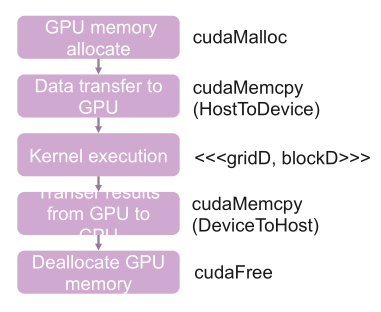
\includegraphics[width=.9\linewidth]{img/cuda_execution.png}
\end{center}
\captionof{figure}{The CUDA execution}\label{fig:the-cuda-execution}
}

\subparagraph{Ceiling Integer} \
\label{sec:org4155746}
\begin{equation}
  \text{#blocks} = \frac{N + (m-1)}{m}
\end{equation}


\begin{equation}
  \text{#blocks} = \frac{N + 1023}{1024}
\end{equation}

\subparagraph{Warp} \
\label{sec:org2b947aa}
A block is internally in \textbf{Warps} allocated.
One Warp consists of 32 Threads.
Each of these 32 threads executeds the same instructions (same branch in same kernel).

{
\begin{center}
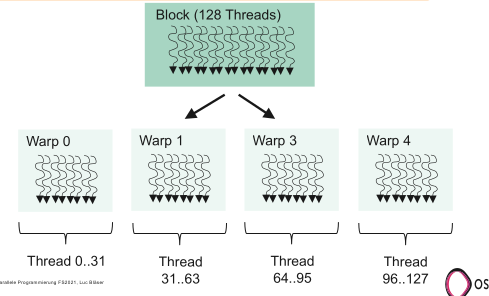
\includegraphics[width=.9\linewidth]{img/block_in_warps.png}
\end{center}
\captionof{figure}{Block in Warp allocated}\label{fig:block-in-warp-allocated}
}

\subparagraph{Memory Coalescing} \
\label{sec:org2f44557}
The pattern how a thread access the memory is critical.
All threads in a warp should access the same ares (burst).
Then a combined access is possible.
Otherwise, you have to do expensive individual accesses.


If you have a an access on memory use always the \texttt{threadIdx.x/y/z} to align the memory access.

\lstset{language=C,label=fig:align-memory-access,caption={Align memory access (coalescing)},captionpos=b,numbers=none}
\begin{lstlisting}
data[(Expression without threadIdx.x) + threadIdx.x]
\end{lstlisting}


\begin{figure}[H]
  \centering
  \begin{subfigure}{0.4\textwidth}
    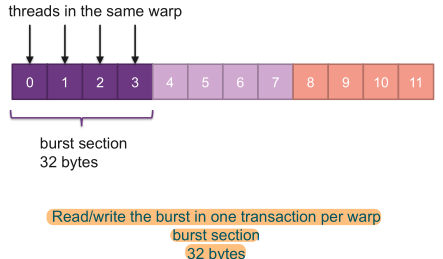
\includegraphics[width=3in]{img/memory_coalescing.png}
    \caption{Memory Coalescing\label{fig:memory-coalescing}}
  \end{subfigure}
  \hfill
  \begin{subfigure}{0.4\textwidth}
    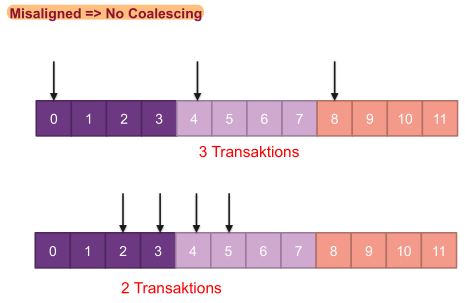
\includegraphics[width=3in]{img/no_memory_coalescing.png}
    \caption{Non-Memory Coalescing\label{fig:non-memory-coalescing}}
  \end{subfigure}
\end{figure}

\subparagraph{CUDA Memory Model} \
\label{sec:orgede2a44}
All threads have access to the same global memory.
Each thread block has shared memory, which is visible to all threads of the block.
The shared memory is much faster because it is on-chip.
The variables in the kernel are normally stored in the regiester (fastest access).
Each thread has private local memory which resides in device memory (slow).
Only when all register are used the GPU uses the local memory.


{
\begin{center}
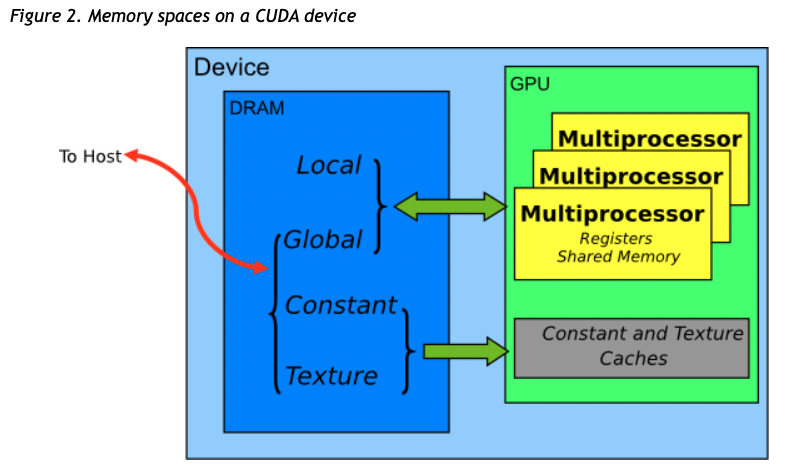
\includegraphics[width=.9\linewidth]{img/simple_memory_model.png}
\end{center}
\captionof{figure}{CUDA memory model}\label{fig:cuda-memory-model}
}

\subparagraph{Shared Memory} \
\label{sec:org6ffdf97}
In matrix multiplication the same row / column is used multiple times.
If the matrix are too big then can not load the whole row / column into memory.
Therefore, the multiplication has to split up.

{
\begin{center}
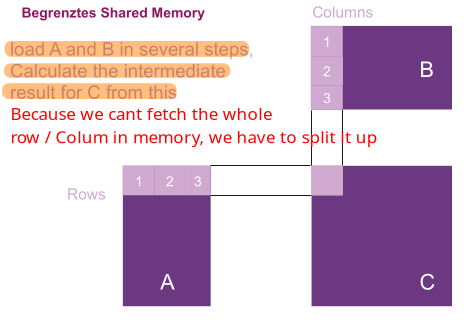
\includegraphics[width=.9\linewidth]{img/tiling_matrix_multiplication.png}
\end{center}
\captionof{figure}{Tiling Matrix Multiplication}\label{fig:tiling-matrix-multiplication}
}

\lstset{language=C,label= ,caption= ,captionpos=b,numbers=none}
\begin{lstlisting}
float sum = 0.0;
for (int tile = 0; tile < nofTiles; tile++) {
  // read tile from a and b in shared memory
  // each thread reads an element from each tile
  __syncthreads();
  // Multiply row of A-Tile by
  // Column of B-Tile from shared memory
  sum += partialProduct;
  __syncthreads();
}
C[row * M + col] = sum;
\end{lstlisting}
\section{Cluster Parallelization}
\label{sec:org6d9b76b}
\section{End}
\label{sec:org29aa14c}
\end{multicols}
\end{document}